\chapter{Problemanalyse}

Det første skridt mod et program er ofte et mockup. Et mockup visualiserer en idé, og får en brainstorm til at være mere konkret. Ud fra dette bliver der arbejdet med hvert enkle element i mockup'en, hvilket ofte gør, at hvert element bliver en klasse i en kode. Ud fra mockup'en er det også lettere at se hvilke klasser skal være forbundet til hinanden, og derefter også hvor data skal placeres (hvis data skal være med).

\section{Beskrivelse}

Vi har valgt at bruge et program (ud af mange) der hedder Balsamiq Mockups.
Det står i problemformuleringen, at Bookie ikke skal være indviklet, hvilket bliver reducéret ti, at Bookie kun skal kunne det mest basale, som et reservationssystem kræver. Data er en nødvendighed, men der er forskellige måder at repræsentere den på.

Ud fra vores mockup, repræsenterer vi data på den måde, at der først bliver valgt en film (\ref{mockup: balsamiq-showtimes}), hvorefter man kommer ind på et vindue, hvor der er muligt at se hvilke dage og tidspunkter den valgte film bliver vist (\ref{mockup: balsamiq-showtimes1}). Inde på næste vindue bliver det så muligt at reservere pladser (\ref{mockup: balsamiq-auditorium}), hvilke så ender inde på \textit{Reservationer} (\ref{mockup: balsamiq-reservation}).

I forhold til vores mockup, er der på startsiden (\ref{mockup: balsamiq-showtimes}) lavet en liste som repræsenterer filmene som data. Til hver film er der en tabel (\ref{mockup: balsamiq-showtimes1}), hvor rækkerne beskriver tidspunkter på dagen, og kolonnerne dagene i ugen. Til hver forestilling er der en sal (\ref{mockup: balsamiq-auditorium}), hvor sæderne er delt op i et gitter, og hvor hvert sæde repræsenterer en billet. Hvilket inkluderer i, at en billet er forbundet med et tidspunkt og en sal, som er forbundet til en film. Dog har \textit{Reservationer} også en liste, men denne liste indeholder billetter. Det vil sige, at billetterne også er forbundet til \textit{Reservationer}, men ikke omvendt.

Inde på \textit{Reservationer} er der også muligt at søge efter en bestemt reservation ved at skrive et telefonnummer ind på \textit{søg}-feltet. Dette felt vil så filtrere numrene i tabellen.

Idéen fungerer fint, men JavaFX har ikke samarbejdet på et optimalt plan, hvilket har fået den endelige brugergrænseflade til at blive lidt anderledes, den har en lidt anden måde at repræsentere data på. Som det også kan ses i \textit{Brugervejledning og eksempel}, så er alle forestillinger i samme tabel, med salene til højre for tabellen. Igen er data fra reservationerne repræsenteret i et gitter. \textit{Reservationer} i Bookie minder meget om mockup'en. 


\subsection{Mockups}

\begin{figure}[h]
  \centering
  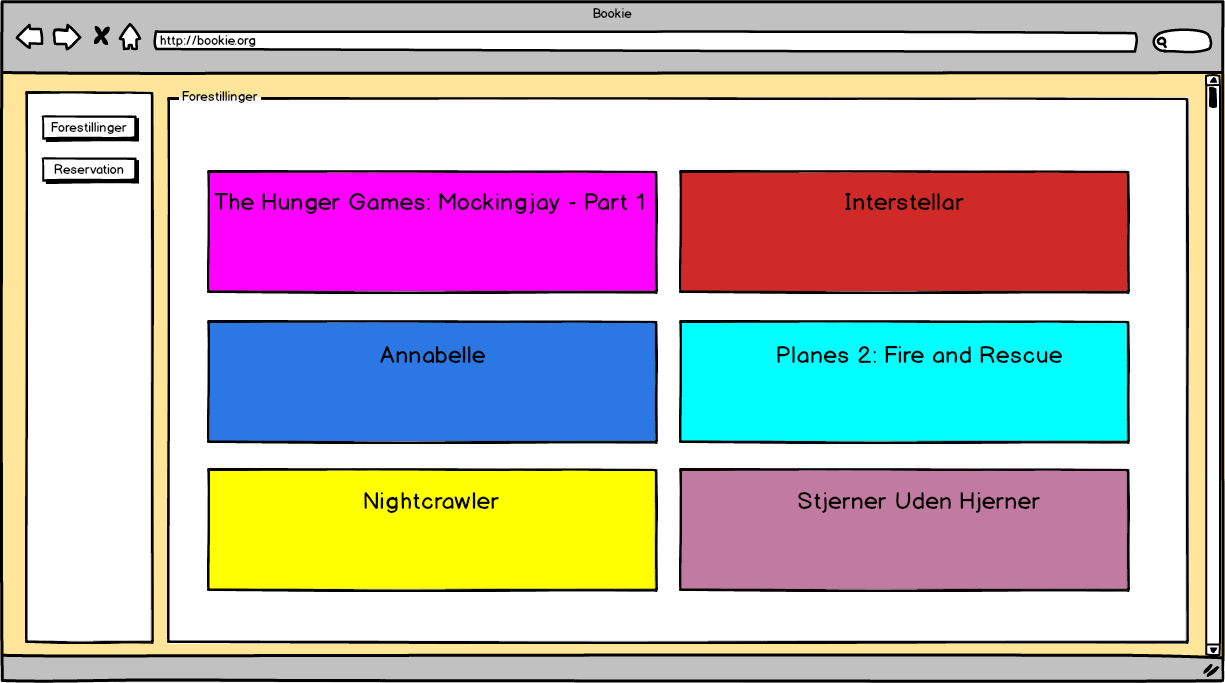
\includegraphics[width=\textwidth]{balsamiq-showtimes.png}
  \caption{Mockup - Bookie startside}
  \label{mockup: balsamiq-showtimes}
\end{figure}

\begin{figure}[h]
  \centering
  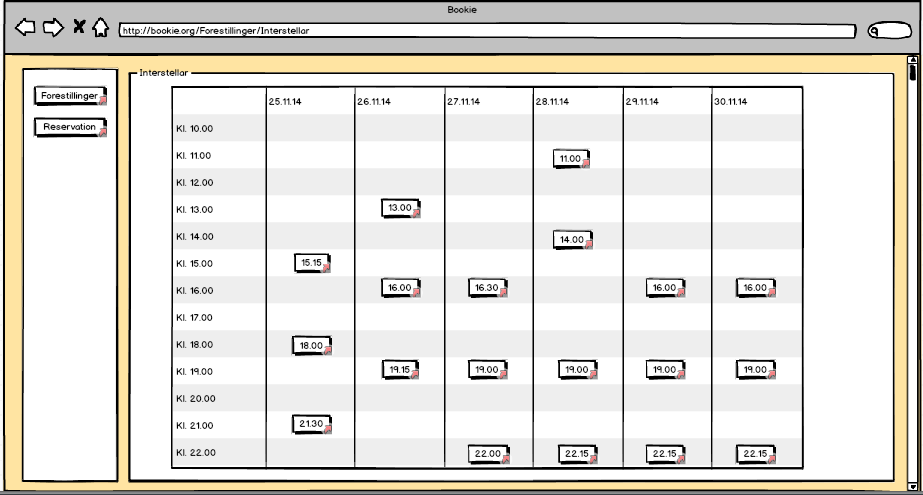
\includegraphics[width=\textwidth]{balsamiq-showtimes1.png}
  \caption{Mockup - tidspunkter}
  \label{mockup: balsamiq-showtimes1}
\end{figure}

\begin{figure}[h]
  \centering
  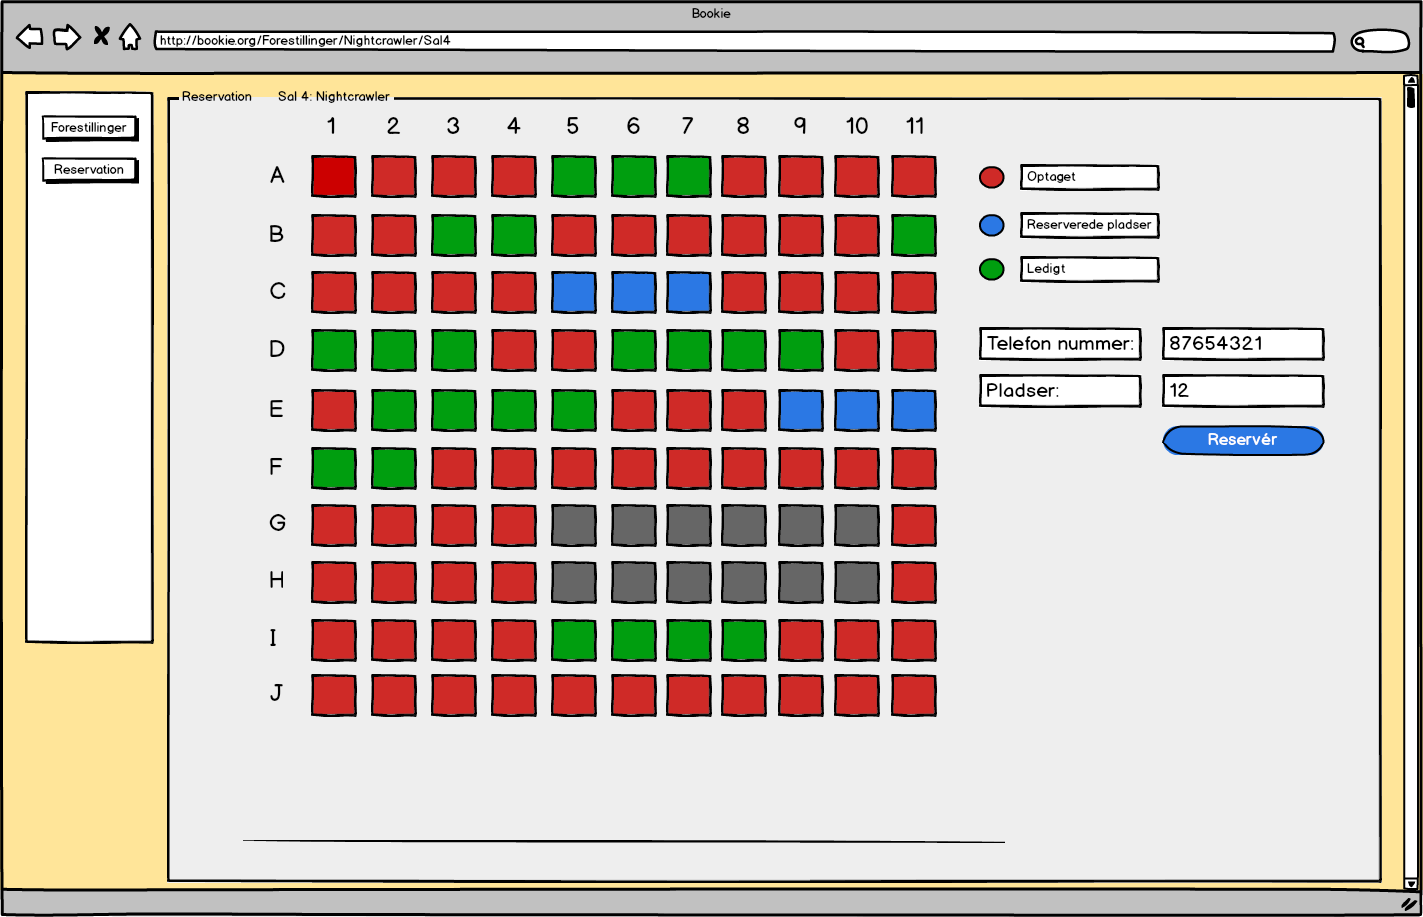
\includegraphics[width=\textwidth]{balsamiq-auditorium.png}
  \caption{Mockup - Eksempel af en sal}
  \label{mockup: balsamiq-auditorium}
\end{figure}

\begin{figure}[h]
  \centering
  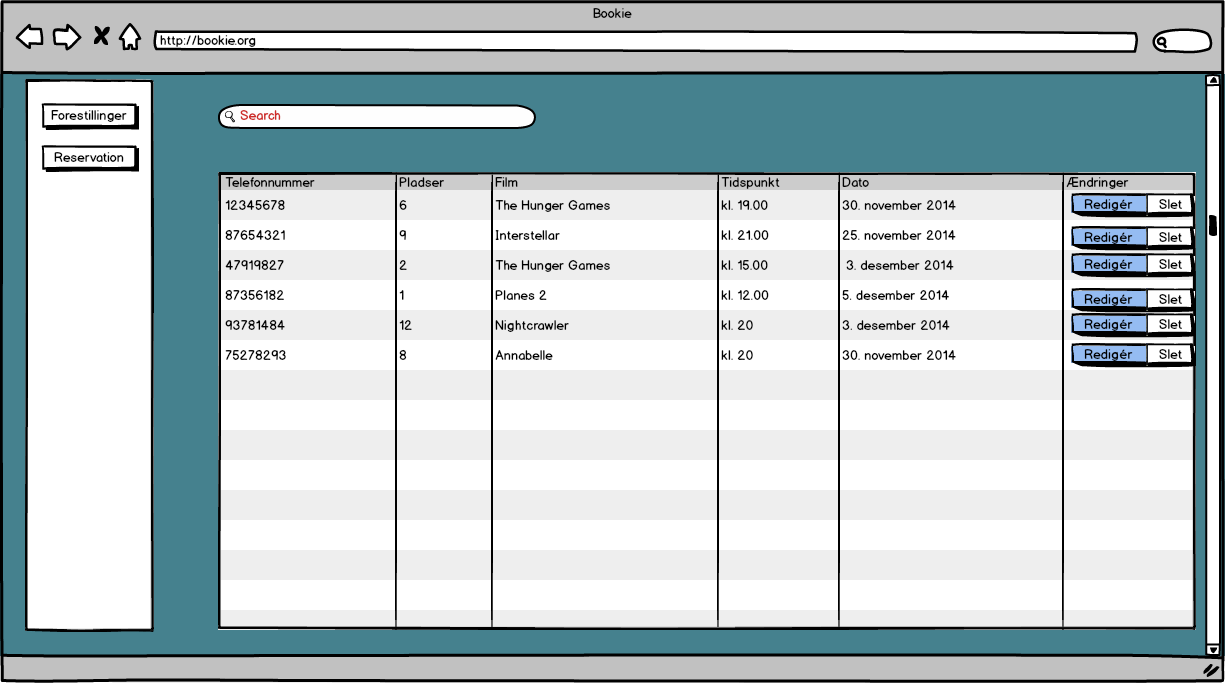
\includegraphics[width=\textwidth]{balsamiq-reservation.png}
  \caption{Mockup - Reservationer}
  \label{mockup: balsamiq-reservation}
\end{figure}

\section{Diskussion}

\section{Databasedesign}

